You are going to estimate the stability margins for the following feedback system
\begin{center}
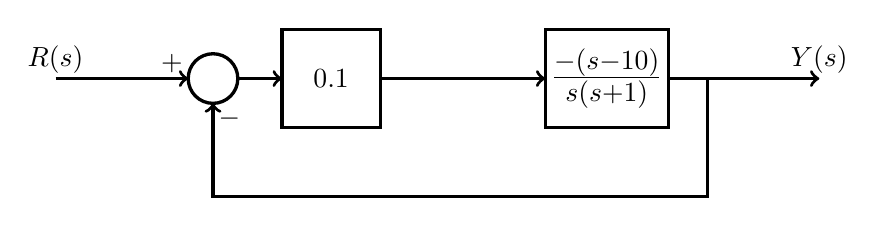
\begin{tikzpicture}[scale=1,inner sep=0pt,outer sep=0pt,very thick,
sysblock/.style={draw,rectangle,inner sep=2pt,minimum width=1.25cm,minimum height=1.25cm,very thick}]
\draw (2,0) node[draw,circle] (sum1) {$\rule{0pt}{18pt}$};
\draw (3.5,0) node[sysblock] (Kp) {$ 0.1$};
\draw (7,0) node[sysblock] (G) {\Large $\frac{-(s-10)}{s(s+1)}$};
\draw[->] (0,0) node[above=2pt] {$R(s)$} -- (sum1.180) node[above left=2pt] {$+$};
\draw[->] (sum1.0) --  (Kp);
\draw[->] (Kp) -- (G);
\draw[->] (G) -- ++(2.7,0) node[above=2pt] {$Y(s)$};
\draw[->] (G.0) ++(.5,0) -- ++(0,-1.5) -| (sum1.-90) node[below right=2pt] {$-$};
\end{tikzpicture}

\end{center}
\begin{enumerate}[(a)]
\item Using the linear approximation rules, sketch the Bode plot for the loop gain
\begin{center}
\includegraphics[width=5in]{\mainfolder/LectureNotes/\lecturefolder/HomeworkProblems/blankbode}
\end{center}
\item Using the information from your sketch, what are the gain margin and phase margin for this feedback system? 
\end{enumerate}
